\documentclass[1p]{elsarticle_modified}
%\bibliographystyle{elsarticle-num}

%\usepackage[colorlinks]{hyperref}
%\usepackage{abbrmath_seonhwa} %\Abb, \Ascr, \Acal ,\Abf, \Afrak
\usepackage{amsfonts}
\usepackage{amssymb}
\usepackage{amsmath}
\usepackage{amsthm}
\usepackage{scalefnt}
\usepackage{amsbsy}
\usepackage{kotex}
\usepackage{caption}
\usepackage{subfig}
\usepackage{color}
\usepackage{graphicx}
\usepackage{xcolor} %% white, black, red, green, blue, cyan, magenta, yellow
\usepackage{float}
\usepackage{setspace}
\usepackage{hyperref}

\usepackage{tikz}
\usetikzlibrary{arrows}

\usepackage{multirow}
\usepackage{array} % fixed length table
\usepackage{hhline}

%%%%%%%%%%%%%%%%%%%%%
\makeatletter
\renewcommand*\env@matrix[1][\arraystretch]{%
	\edef\arraystretch{#1}%
	\hskip -\arraycolsep
	\let\@ifnextchar\new@ifnextchar
	\array{*\c@MaxMatrixCols c}}
\makeatother %https://tex.stackexchange.com/questions/14071/how-can-i-increase-the-line-spacing-in-a-matrix
%%%%%%%%%%%%%%%

\usepackage[normalem]{ulem}

\newcommand{\msout}[1]{\ifmmode\text{\sout{\ensuremath{#1}}}\else\sout{#1}\fi}
%SOURCE: \msout is \stkout macro in https://tex.stackexchange.com/questions/20609/strikeout-in-math-mode

\newcommand{\cancel}[1]{
	\ifmmode
	{\color{red}\msout{#1}}
	\else
	{\color{red}\sout{#1}}
	\fi
}

\newcommand{\add}[1]{
	{\color{blue}\uwave{#1}}
}

\newcommand{\replace}[2]{
	\ifmmode
	{\color{red}\msout{#1}}{\color{blue}\uwave{#2}}
	\else
	{\color{red}\sout{#1}}{\color{blue}\uwave{#2}}
	\fi
}

\newcommand{\Sol}{\mathcal{S}} %segment
\newcommand{\D}{D} %diagram
\newcommand{\A}{\mathcal{A}} %arc


%%%%%%%%%%%%%%%%%%%%%%%%%%%%%5 test

\def\sl{\operatorname{\textup{SL}}(2,\Cbb)}
\def\psl{\operatorname{\textup{PSL}}(2,\Cbb)}
\def\quan{\mkern 1mu \triangleright \mkern 1mu}

\theoremstyle{definition}
\newtheorem{thm}{Theorem}[section]
\newtheorem{prop}[thm]{Proposition}
\newtheorem{lem}[thm]{Lemma}
\newtheorem{ques}[thm]{Question}
\newtheorem{cor}[thm]{Corollary}
\newtheorem{defn}[thm]{Definition}
\newtheorem{exam}[thm]{Example}
\newtheorem{rmk}[thm]{Remark}
\newtheorem{alg}[thm]{Algorithm}

\newcommand{\I}{\sqrt{-1}}
\begin{document}

%\begin{frontmatter}
%
%\title{Boundary parabolic representations of knots up to 8 crossings}
%
%%% Group authors per affiliation:
%\author{Yunhi Cho} 
%\address{Department of Mathematics, University of Seoul, Seoul, Korea}
%\ead{yhcho@uos.ac.kr}
%
%
%\author{Seonhwa Kim} %\fnref{s_kim}}
%\address{Center for Geometry and Physics, Institute for Basic Science, Pohang, 37673, Korea}
%\ead{ryeona17@ibs.re.kr}
%
%\author{Hyuk Kim}
%\address{Department of Mathematical Sciences, Seoul National University, Seoul 08826, Korea}
%\ead{hyukkim@snu.ac.kr}
%
%\author{Seokbeom Yoon}
%\address{Department of Mathematical Sciences, Seoul National University, Seoul, 08826,  Korea}
%\ead{sbyoon15@snu.ac.kr}
%
%\begin{abstract}
%We find all boundary parabolic representation of knots up to 8 crossings.
%
%\end{abstract}
%\begin{keyword}
%    \MSC[2010] 57M25 
%\end{keyword}
%
%\end{frontmatter}

%\linenumbers
%\tableofcontents
%
\newcommand\colored[1]{\textcolor{white}{\rule[-0.35ex]{0.8em}{1.4ex}}\kern-0.8em\color{red} #1}%
%\newcommand\colored[1]{\textcolor{white}{ #1}\kern-2.17ex	\textcolor{white}{ #1}\kern-1.81ex	\textcolor{white}{ #1}\kern-2.15ex\color{red}#1	}

{\Large $\underline{12a_{0714}~(K12a_{0714})}$}

\setlength{\tabcolsep}{10pt}
\renewcommand{\arraystretch}{1.6}
\vspace{1cm}\begin{tabular}{m{100pt}>{\centering\arraybackslash}m{274pt}}
\multirow{5}{120pt}{
	\centering
	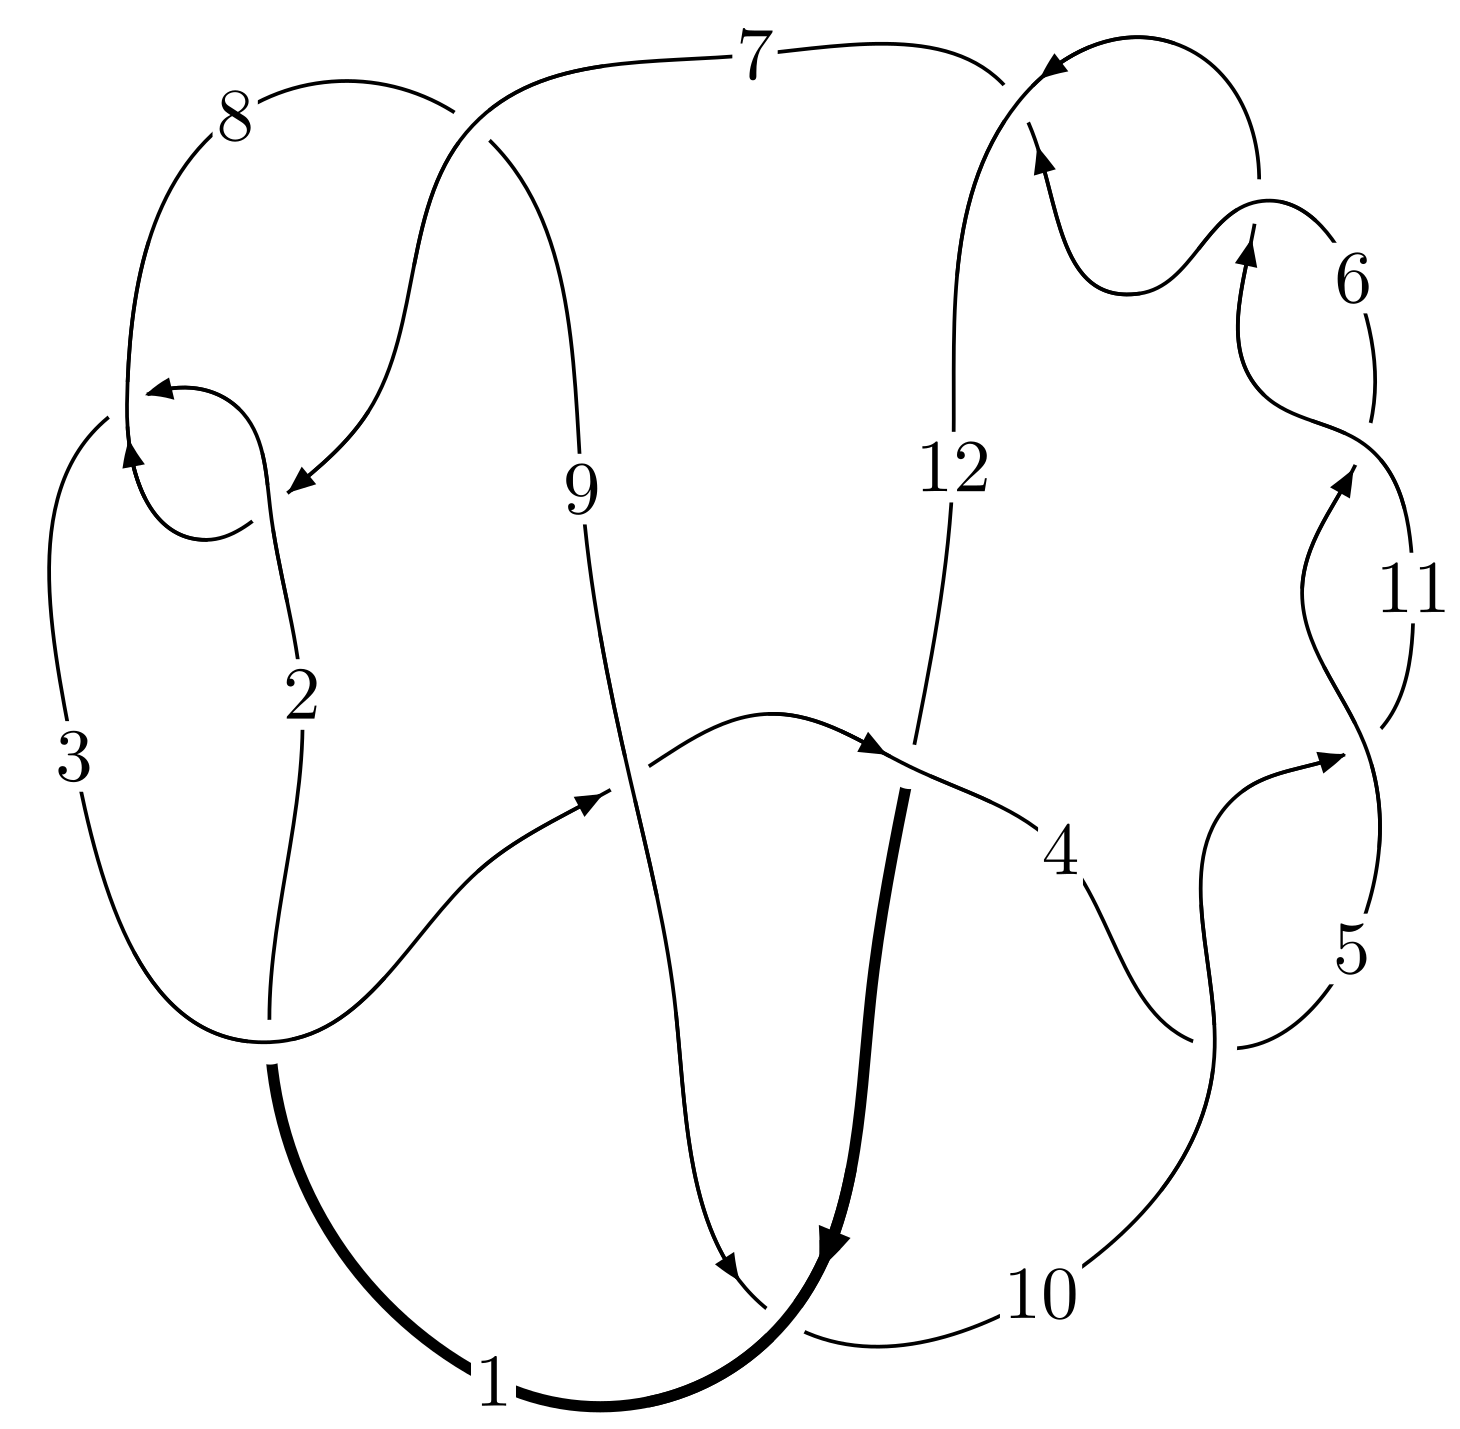
\includegraphics[width=112pt]{../../../GIT/diagram.site/Diagrams/png/1515_12a_0714.png}\\
\ \ \ A knot diagram\footnotemark}&
\allowdisplaybreaks
\textbf{Linearized knot diagam} \\
\cline{2-2}
 &
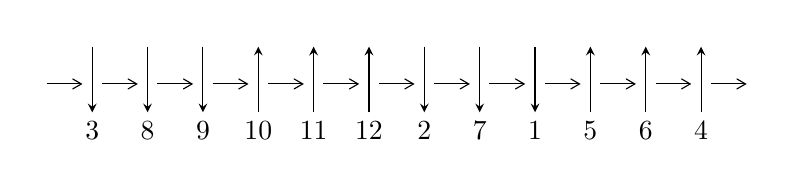
\begin{tikzpicture}[x=20pt, y=17pt]
	% nodes
	\node (C0) at (0, 0) {};
	\node (C1) at (1, 0) {};
	\node (C1U) at (1, +1) {};
	\node (C1D) at (1, -1) {3};

	\node (C2) at (2, 0) {};
	\node (C2U) at (2, +1) {};
	\node (C2D) at (2, -1) {8};

	\node (C3) at (3, 0) {};
	\node (C3U) at (3, +1) {};
	\node (C3D) at (3, -1) {9};

	\node (C4) at (4, 0) {};
	\node (C4U) at (4, +1) {};
	\node (C4D) at (4, -1) {10};

	\node (C5) at (5, 0) {};
	\node (C5U) at (5, +1) {};
	\node (C5D) at (5, -1) {11};

	\node (C6) at (6, 0) {};
	\node (C6U) at (6, +1) {};
	\node (C6D) at (6, -1) {12};

	\node (C7) at (7, 0) {};
	\node (C7U) at (7, +1) {};
	\node (C7D) at (7, -1) {2};

	\node (C8) at (8, 0) {};
	\node (C8U) at (8, +1) {};
	\node (C8D) at (8, -1) {7};

	\node (C9) at (9, 0) {};
	\node (C9U) at (9, +1) {};
	\node (C9D) at (9, -1) {1};

	\node (C10) at (10, 0) {};
	\node (C10U) at (10, +1) {};
	\node (C10D) at (10, -1) {5};

	\node (C11) at (11, 0) {};
	\node (C11U) at (11, +1) {};
	\node (C11D) at (11, -1) {6};

	\node (C12) at (12, 0) {};
	\node (C12U) at (12, +1) {};
	\node (C12D) at (12, -1) {4};
	\node (C13) at (13, 0) {};

	% arrows
	\draw[->,>={angle 60}]
	(C0) edge (C1) (C1) edge (C2) (C2) edge (C3) (C3) edge (C4) (C4) edge (C5) (C5) edge (C6) (C6) edge (C7) (C7) edge (C8) (C8) edge (C9) (C9) edge (C10) (C10) edge (C11) (C11) edge (C12) (C12) edge (C13) ;	\draw[->,>=stealth]
	(C1U) edge (C1D) (C2U) edge (C2D) (C3U) edge (C3D) (C4D) edge (C4U) (C5D) edge (C5U) (C6D) edge (C6U) (C7U) edge (C7D) (C8U) edge (C8D) (C9U) edge (C9D) (C10D) edge (C10U) (C11D) edge (C11U) (C12D) edge (C12U) ;
	\end{tikzpicture} \\
\hhline{~~} \\& 
\textbf{Solving Sequence} \\ \cline{2-2} 
 &
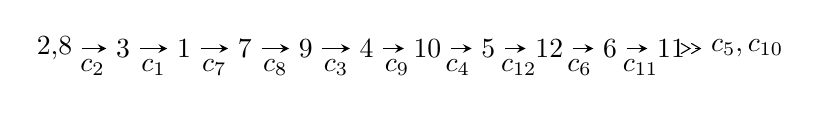
\begin{tikzpicture}[x=22pt, y=7pt]
	% node
	\node (A0) at (-1/8, 0) {2,8};
	\node (A1) at (1, 0) {3};
	\node (A2) at (2, 0) {1};
	\node (A3) at (3, 0) {7};
	\node (A4) at (4, 0) {9};
	\node (A5) at (5, 0) {4};
	\node (A6) at (6, 0) {10};
	\node (A7) at (7, 0) {5};
	\node (A8) at (8, 0) {12};
	\node (A9) at (9, 0) {6};
	\node (A10) at (10, 0) {11};
	\node (C1) at (1/2, -1) {$c_{2}$};
	\node (C2) at (3/2, -1) {$c_{1}$};
	\node (C3) at (5/2, -1) {$c_{7}$};
	\node (C4) at (7/2, -1) {$c_{8}$};
	\node (C5) at (9/2, -1) {$c_{3}$};
	\node (C6) at (11/2, -1) {$c_{9}$};
	\node (C7) at (13/2, -1) {$c_{4}$};
	\node (C8) at (15/2, -1) {$c_{12}$};
	\node (C9) at (17/2, -1) {$c_{6}$};
	\node (C10) at (19/2, -1) {$c_{11}$};
	\node (A11) at (45/4, 0) {$c_{5},c_{10}$};

	% edge
	\draw[->,>=stealth]	
	(A0) edge (A1) (A1) edge (A2) (A2) edge (A3) (A3) edge (A4) (A4) edge (A5) (A5) edge (A6) (A6) edge (A7) (A7) edge (A8) (A8) edge (A9) (A9) edge (A10) ;
	\draw[->>,>={angle 60}]	
	(A10) edge (A11);
\end{tikzpicture} \\ 

\end{tabular} \\

\footnotetext{
The image of knot diagram is generated by the software ``\textbf{Draw programme}" developed by Andrew Bartholomew(\url{http://www.layer8.co.uk/maths/draw/index.htm\#Running-draw}), where we modified some parts for our purpose(\url{https://github.com/CATsTAILs/LinksPainter}).
}\phantom \\ \newline 
\centering \textbf{Ideals for irreducible components\footnotemark of $X_{\text{par}}$} 
 
\begin{align*}
I^u_{1}&=\langle 
u^{53}+u^{52}+\cdots- u-1\rangle \\
\\
\end{align*}
\raggedright * 1 irreducible components of $\dim_{\mathbb{C}}=0$, with total 53 representations.\\
\footnotetext{All coefficients of polynomials are rational numbers. But the coefficients are sometimes approximated in decimal forms when there is not enough margin.}
\newpage
\renewcommand{\arraystretch}{1}
\centering \section*{I. $I^u_{1}= \langle u^{53}+u^{52}+\cdots- u-1 \rangle$}
\flushleft \textbf{(i) Arc colorings}\\
\begin{tabular}{m{7pt} m{180pt} m{7pt} m{180pt} }
\flushright $a_{2}=$&$\begin{pmatrix}1\\0\end{pmatrix}$ \\
\flushright $a_{8}=$&$\begin{pmatrix}0\\u\end{pmatrix}$ \\
\flushright $a_{3}=$&$\begin{pmatrix}1\\u^2\end{pmatrix}$ \\
\flushright $a_{1}=$&$\begin{pmatrix}- u^2+1\\- u^4\end{pmatrix}$ \\
\flushright $a_{7}=$&$\begin{pmatrix}u\\u\end{pmatrix}$ \\
\flushright $a_{9}=$&$\begin{pmatrix}- u^3\\- u^3+u\end{pmatrix}$ \\
\flushright $a_{4}=$&$\begin{pmatrix}- u^8+u^6- u^4+1\\- u^8+2 u^6-2 u^4+2 u^2\end{pmatrix}$ \\
\flushright $a_{10}=$&$\begin{pmatrix}- u^9+2 u^7-3 u^5+2 u^3- u\\- u^{11}+u^9-2 u^7+u^5- u^3+u\end{pmatrix}$ \\
\flushright $a_{5}=$&$\begin{pmatrix}u^{28}-5 u^{26}+\cdots+u^2+1\\u^{30}-4 u^{28}+\cdots-2 u^4+u^2\end{pmatrix}$ \\
\flushright $a_{12}=$&$\begin{pmatrix}u^{20}-3 u^{18}+7 u^{16}-10 u^{14}+10 u^{12}-7 u^{10}+u^8+2 u^6-3 u^4+u^2+1\\u^{20}-4 u^{18}+10 u^{16}-18 u^{14}+23 u^{12}-24 u^{10}+18 u^8-10 u^6+3 u^4\end{pmatrix}$ \\
\flushright $a_{6}=$&$\begin{pmatrix}- u^{39}+6 u^{37}+\cdots+8 u^5-2 u^3\\- u^{39}+7 u^{37}+\cdots-3 u^5+u\end{pmatrix}$ \\
\flushright $a_{11}=$&$\begin{pmatrix}u^{47}-8 u^{45}+\cdots-10 u^5+4 u^3\\u^{49}-7 u^{47}+\cdots-2 u^7+u\end{pmatrix}$\\&\end{tabular}
\flushleft \textbf{(ii) Obstruction class $= -1$}\\~\\
\flushleft \textbf{(iii) Cusp Shapes $= 4 u^{52}-36 u^{50}+\cdots-8 u-2$}\\~\\
\newpage\renewcommand{\arraystretch}{1}
\flushleft \textbf{(iv) u-Polynomials at the component}\newline \\
\begin{tabular}{m{50pt}|m{274pt}}
Crossings & \hspace{64pt}u-Polynomials at each crossing \\
\hline $$\begin{aligned}c_{1},c_{8}\end{aligned}$$&$\begin{aligned}
&u^{53}+17 u^{52}+\cdots- u+1
\end{aligned}$\\
\hline $$\begin{aligned}c_{2},c_{7}\end{aligned}$$&$\begin{aligned}
&u^{53}+u^{52}+\cdots- u-1
\end{aligned}$\\
\hline $$\begin{aligned}c_{3}\end{aligned}$$&$\begin{aligned}
&u^{53}- u^{52}+\cdots+13 u-1
\end{aligned}$\\
\hline $$\begin{aligned}c_{4},c_{5},c_{6}\\c_{10},c_{11}\end{aligned}$$&$\begin{aligned}
&u^{53}+u^{52}+\cdots- u-1
\end{aligned}$\\
\hline $$\begin{aligned}c_{9}\end{aligned}$$&$\begin{aligned}
&u^{53}+7 u^{52}+\cdots+293 u+295
\end{aligned}$\\
\hline $$\begin{aligned}c_{12}\end{aligned}$$&$\begin{aligned}
&u^{53}+5 u^{52}+\cdots-417 u-99
\end{aligned}$\\
\hline
\end{tabular}\\~\\
\newpage\renewcommand{\arraystretch}{1}
\flushleft \textbf{(v) Riley Polynomials at the component}\newline \\
\begin{tabular}{m{50pt}|m{274pt}}
Crossings & \hspace{64pt}Riley Polynomials at each crossing \\
\hline $$\begin{aligned}c_{1},c_{8}\end{aligned}$$&$\begin{aligned}
&y^{53}+39 y^{52}+\cdots+19 y-1
\end{aligned}$\\
\hline $$\begin{aligned}c_{2},c_{7}\end{aligned}$$&$\begin{aligned}
&y^{53}-17 y^{52}+\cdots- y-1
\end{aligned}$\\
\hline $$\begin{aligned}c_{3}\end{aligned}$$&$\begin{aligned}
&y^{53}+3 y^{52}+\cdots+47 y-1
\end{aligned}$\\
\hline $$\begin{aligned}c_{4},c_{5},c_{6}\\c_{10},c_{11}\end{aligned}$$&$\begin{aligned}
&y^{53}-69 y^{52}+\cdots- y-1
\end{aligned}$\\
\hline $$\begin{aligned}c_{9}\end{aligned}$$&$\begin{aligned}
&y^{53}+23 y^{52}+\cdots-620381 y-87025
\end{aligned}$\\
\hline $$\begin{aligned}c_{12}\end{aligned}$$&$\begin{aligned}
&y^{53}-13 y^{52}+\cdots+120231 y-9801
\end{aligned}$\\
\hline
\end{tabular}\\~\\
\newpage\flushleft \textbf{(vi) Complex Volumes and Cusp Shapes}
$$\begin{array}{c|c|c}  
\text{Solutions to }I^u_{1}& \I (\text{vol} + \sqrt{-1}CS) & \text{Cusp shape}\\
 \hline 
\begin{aligned}
u &= -0.917964 + 0.396458 I\end{aligned}
 & \phantom{-}11.02350 - 1.17650 I & \phantom{-}3.47656 - 1.29829 I \\ \hline\begin{aligned}
u &= -0.917964 - 0.396458 I\end{aligned}
 & \phantom{-}11.02350 + 1.17650 I & \phantom{-}3.47656 + 1.29829 I \\ \hline\begin{aligned}
u &= \phantom{-}1.004410 + 0.120149 I\end{aligned}
 & -3.30847 - 2.92968 I & -6.10401 + 5.98646 I \\ \hline\begin{aligned}
u &= \phantom{-}1.004410 - 0.120149 I\end{aligned}
 & -3.30847 + 2.92968 I & -6.10401 - 5.98646 I \\ \hline\begin{aligned}
u &= -0.965969 + 0.058477 I\end{aligned}
 & -2.10934 + 0.19404 I & -2.74556 + 1.38490 I \\ \hline\begin{aligned}
u &= -0.965969 - 0.058477 I\end{aligned}
 & -2.10934 - 0.19404 I & -2.74556 - 1.38490 I \\ \hline\begin{aligned}
u &= -1.026680 + 0.154387 I\end{aligned}
 & \phantom{-}0.16153 + 5.66463 I & \phantom{-}0.36927 - 7.13482 I \\ \hline\begin{aligned}
u &= -1.026680 - 0.154387 I\end{aligned}
 & \phantom{-}0.16153 - 5.66463 I & \phantom{-}0.36927 + 7.13482 I \\ \hline\begin{aligned}
u &= \phantom{-}1.03975\phantom{ +0.000000I}\end{aligned}
 & \phantom{-}5.77807\phantom{ +0.000000I} & -1.63810\phantom{ +0.000000I} \\ \hline\begin{aligned}
u &= \phantom{-}0.808317 + 0.497173 I\end{aligned}
 & \phantom{-}1.80074 + 0.19940 I & \phantom{-}3.10423 - 0.79204 I \\ \hline\begin{aligned}
u &= \phantom{-}0.808317 - 0.497173 I\end{aligned}
 & \phantom{-}1.80074 - 0.19940 I & \phantom{-}3.10423 + 0.79204 I \\ \hline\begin{aligned}
u &= \phantom{-}1.045770 + 0.171126 I\end{aligned}
 & \phantom{-}9.64765 - 7.13925 I & \phantom{-}1.62928 + 5.46600 I \\ \hline\begin{aligned}
u &= \phantom{-}1.045770 - 0.171126 I\end{aligned}
 & \phantom{-}9.64765 + 7.13925 I & \phantom{-}1.62928 - 5.46600 I \\ \hline\begin{aligned}
u &= -0.711976 + 0.788691 I\end{aligned}
 & \phantom{-}2.77377 - 2.54983 I & \phantom{-}2.56238 + 3.84090 I \\ \hline\begin{aligned}
u &= -0.711976 - 0.788691 I\end{aligned}
 & \phantom{-}2.77377 + 2.54983 I & \phantom{-}2.56238 - 3.84090 I \\ \hline\begin{aligned}
u &= \phantom{-}0.741129 + 0.766184 I\end{aligned}
 & \phantom{-}3.37856 - 0.51833 I & \phantom{-}4.74330 + 3.74158 I \\ \hline\begin{aligned}
u &= \phantom{-}0.741129 - 0.766184 I\end{aligned}
 & \phantom{-}3.37856 + 0.51833 I & \phantom{-}4.74330 - 3.74158 I \\ \hline\begin{aligned}
u &= -0.898334 + 0.585827 I\end{aligned}
 & -0.89223 + 2.27300 I & -4.11058 - 2.34862 I \\ \hline\begin{aligned}
u &= -0.898334 - 0.585827 I\end{aligned}
 & -0.89223 - 2.27300 I & -4.11058 + 2.34862 I \\ \hline\begin{aligned}
u &= \phantom{-}0.706508 + 0.812636 I\end{aligned}
 & \phantom{-}6.62164 + 5.35410 I & \phantom{-}7.68244 - 4.25676 I \\ \hline\begin{aligned}
u &= \phantom{-}0.706508 - 0.812636 I\end{aligned}
 & \phantom{-}6.62164 - 5.35410 I & \phantom{-}7.68244 + 4.25676 I \\ \hline\begin{aligned}
u &= -0.703816 + 0.827557 I\end{aligned}
 & \phantom{-}16.3321 - 6.9044 I & \phantom{-}8.55087 + 2.77192 I \\ \hline\begin{aligned}
u &= -0.703816 - 0.827557 I\end{aligned}
 & \phantom{-}16.3321 + 6.9044 I & \phantom{-}8.55087 - 2.77192 I \\ \hline\begin{aligned}
u &= -0.780598 + 0.788930 I\end{aligned}
 & \phantom{-}7.91993 + 2.45268 I & \phantom{-}9.54638 - 3.47883 I \\ \hline\begin{aligned}
u &= -0.780598 - 0.788930 I\end{aligned}
 & \phantom{-}7.91993 - 2.45268 I & \phantom{-}9.54638 + 3.47883 I \\ \hline\begin{aligned}
u &= \phantom{-}0.941389 + 0.627556 I\end{aligned}
 & \phantom{-}1.18896 - 4.90002 I & \phantom{-}2.00262 + 7.53056 I \\ \hline\begin{aligned}
u &= \phantom{-}0.941389 - 0.627556 I\end{aligned}
 & \phantom{-}1.18896 + 4.90002 I & \phantom{-}2.00262 - 7.53056 I \\ \hline\begin{aligned}
u &= \phantom{-}0.792770 + 0.808036 I\end{aligned}
 & \phantom{-}17.9061 - 3.4233 I & \phantom{-}9.92605 + 2.63045 I \\ \hline\begin{aligned}
u &= \phantom{-}0.792770 - 0.808036 I\end{aligned}
 & \phantom{-}17.9061 + 3.4233 I & \phantom{-}9.92605 - 2.63045 I \\ \hline\begin{aligned}
u &= -0.567997 + 0.619087 I\end{aligned}
 & \phantom{-}10.69110 - 0.81715 I & \phantom{-}5.56596 - 0.12172 I\\
 \hline 
 \end{array}$$\newpage$$\begin{array}{c|c|c}  
\text{Solutions to }I^u_{1}& \I (\text{vol} + \sqrt{-1}CS) & \text{Cusp shape}\\
 \hline 
\begin{aligned}
u &= -0.567997 - 0.619087 I\end{aligned}
 & \phantom{-}10.69110 + 0.81715 I & \phantom{-}5.56596 + 0.12172 I \\ \hline\begin{aligned}
u &= -0.984073 + 0.636487 I\end{aligned}
 & \phantom{-}9.59431 + 5.77095 I & \phantom{-0.000000 } 0. - 5.49289 I \\ \hline\begin{aligned}
u &= -0.984073 - 0.636487 I\end{aligned}
 & \phantom{-}9.59431 - 5.77095 I & \phantom{-0.000000 -}0. + 5.49289 I \\ \hline\begin{aligned}
u &= -0.952798 + 0.740289 I\end{aligned}
 & \phantom{-}7.39031 + 3.31063 I & \phantom{-0.000000 } 0 \\ \hline\begin{aligned}
u &= -0.952798 - 0.740289 I\end{aligned}
 & \phantom{-}7.39031 - 3.31063 I & \phantom{-0.000000 } 0 \\ \hline\begin{aligned}
u &= \phantom{-}0.974166 + 0.713810 I\end{aligned}
 & \phantom{-}2.66592 - 5.09809 I & \phantom{-0.000000 } 0 \\ \hline\begin{aligned}
u &= \phantom{-}0.974166 - 0.713810 I\end{aligned}
 & \phantom{-}2.66592 + 5.09809 I & \phantom{-0.000000 } 0 \\ \hline\begin{aligned}
u &= \phantom{-}0.952090 + 0.759043 I\end{aligned}
 & \phantom{-}17.4152 - 2.4557 I & \phantom{-0.000000 } 0 \\ \hline\begin{aligned}
u &= \phantom{-}0.952090 - 0.759043 I\end{aligned}
 & \phantom{-}17.4152 + 2.4557 I & \phantom{-0.000000 } 0 \\ \hline\begin{aligned}
u &= -0.994703 + 0.718854 I\end{aligned}
 & \phantom{-}1.91508 + 8.24431 I & \phantom{-0.000000 } 0 \\ \hline\begin{aligned}
u &= -0.994703 - 0.718854 I\end{aligned}
 & \phantom{-}1.91508 - 8.24431 I & \phantom{-0.000000 } 0 \\ \hline\begin{aligned}
u &= \phantom{-}1.005020 + 0.728341 I\end{aligned}
 & \phantom{-}5.71195 - 11.14500 I & \phantom{-0.000000 } 0 \\ \hline\begin{aligned}
u &= \phantom{-}1.005020 - 0.728341 I\end{aligned}
 & \phantom{-}5.71195 + 11.14500 I & \phantom{-0.000000 } 0 \\ \hline\begin{aligned}
u &= \phantom{-}0.654395 + 0.369401 I\end{aligned}
 & \phantom{-}1.81787 + 0.23650 I & \phantom{-}4.15811 + 0.08826 I \\ \hline\begin{aligned}
u &= \phantom{-}0.654395 - 0.369401 I\end{aligned}
 & \phantom{-}1.81787 - 0.23650 I & \phantom{-}4.15811 - 0.08826 I \\ \hline\begin{aligned}
u &= -1.011890 + 0.734334 I\end{aligned}
 & \phantom{-}15.3906 + 12.7564 I & \phantom{-0.000000 } 0 \\ \hline\begin{aligned}
u &= -1.011890 - 0.734334 I\end{aligned}
 & \phantom{-}15.3906 - 12.7564 I & \phantom{-0.000000 } 0 \\ \hline\begin{aligned}
u &= -0.124769 + 0.640044 I\end{aligned}
 & \phantom{-}13.4136 + 4.6017 I & \phantom{-}8.93924 - 3.30114 I \\ \hline\begin{aligned}
u &= -0.124769 - 0.640044 I\end{aligned}
 & \phantom{-}13.4136 - 4.6017 I & \phantom{-}8.93924 + 3.30114 I \\ \hline\begin{aligned}
u &= \phantom{-}0.124451 + 0.589584 I\end{aligned}
 & \phantom{-}3.80539 - 3.34966 I & \phantom{-}8.46314 + 5.01124 I \\ \hline\begin{aligned}
u &= \phantom{-}0.124451 - 0.589584 I\end{aligned}
 & \phantom{-}3.80539 + 3.34966 I & \phantom{-}8.46314 - 5.01124 I \\ \hline\begin{aligned}
u &= -0.128727 + 0.466132 I\end{aligned}
 & \phantom{-}0.171113 + 1.087940 I & \phantom{-}2.68023 - 5.97711 I \\ \hline\begin{aligned}
u &= -0.128727 - 0.466132 I\end{aligned}
 & \phantom{-}0.171113 - 1.087940 I & \phantom{-}2.68023 + 5.97711 I\\
 \hline 
 \end{array}$$\newpage
\newpage\renewcommand{\arraystretch}{1}
\centering \section*{ II. u-Polynomials}
\begin{tabular}{m{50pt}|m{274pt}}
Crossings & \hspace{64pt}u-Polynomials at each crossing \\
\hline $$\begin{aligned}c_{1},c_{8}\end{aligned}$$&$\begin{aligned}
&u^{53}+17 u^{52}+\cdots- u+1
\end{aligned}$\\
\hline $$\begin{aligned}c_{2},c_{7}\end{aligned}$$&$\begin{aligned}
&u^{53}+u^{52}+\cdots- u-1
\end{aligned}$\\
\hline $$\begin{aligned}c_{3}\end{aligned}$$&$\begin{aligned}
&u^{53}- u^{52}+\cdots+13 u-1
\end{aligned}$\\
\hline $$\begin{aligned}c_{4},c_{5},c_{6}\\c_{10},c_{11}\end{aligned}$$&$\begin{aligned}
&u^{53}+u^{52}+\cdots- u-1
\end{aligned}$\\
\hline $$\begin{aligned}c_{9}\end{aligned}$$&$\begin{aligned}
&u^{53}+7 u^{52}+\cdots+293 u+295
\end{aligned}$\\
\hline $$\begin{aligned}c_{12}\end{aligned}$$&$\begin{aligned}
&u^{53}+5 u^{52}+\cdots-417 u-99
\end{aligned}$\\
\hline
\end{tabular}\newpage\renewcommand{\arraystretch}{1}
\centering \section*{ III. Riley Polynomials}
\begin{tabular}{m{50pt}|m{274pt}}
Crossings & \hspace{64pt}Riley Polynomials at each crossing \\
\hline $$\begin{aligned}c_{1},c_{8}\end{aligned}$$&$\begin{aligned}
&y^{53}+39 y^{52}+\cdots+19 y-1
\end{aligned}$\\
\hline $$\begin{aligned}c_{2},c_{7}\end{aligned}$$&$\begin{aligned}
&y^{53}-17 y^{52}+\cdots- y-1
\end{aligned}$\\
\hline $$\begin{aligned}c_{3}\end{aligned}$$&$\begin{aligned}
&y^{53}+3 y^{52}+\cdots+47 y-1
\end{aligned}$\\
\hline $$\begin{aligned}c_{4},c_{5},c_{6}\\c_{10},c_{11}\end{aligned}$$&$\begin{aligned}
&y^{53}-69 y^{52}+\cdots- y-1
\end{aligned}$\\
\hline $$\begin{aligned}c_{9}\end{aligned}$$&$\begin{aligned}
&y^{53}+23 y^{52}+\cdots-620381 y-87025
\end{aligned}$\\
\hline $$\begin{aligned}c_{12}\end{aligned}$$&$\begin{aligned}
&y^{53}-13 y^{52}+\cdots+120231 y-9801
\end{aligned}$\\
\hline
\end{tabular}
\vskip 2pc
\end{document}